\begin{multicols}{2}

\section{Ondes mécaniques}

\subsection{Ondes mécaniques -exemples et définition }

Au premier chapitre, nous avons vu les caractéristiques des oscillateurs
harmoniques.

Un oscillateur harmonique vibrant au sein d'un milieu produit une onde
au sein de ce milieu. Mais qu'est-ce qu'une onde~?

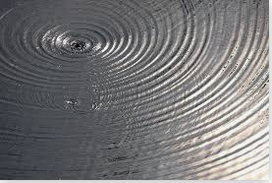
\includegraphics[width=4.032cm,height=2.711cm]{Pictures/1000000100000110000000B7020F4AB269606603.png}

Prenons quelques exemples~:

\begin{itemize}
\item  Laissez tomber un caillou dans l'eau, la chute du caillou dans l'eau
  produit des vagues. Ces vagues se propagent au sein du milieu (ici
  l'eau). Dans ce cas, l'oscillateur harmonique est du à la chute du
  caillou et l'onde est due aux vagues qui se propagent.
   \begin{figure}
   \centering
   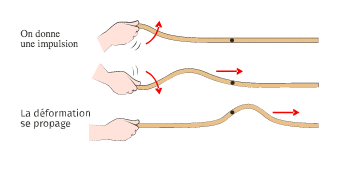
\includegraphics[width=6.01cm,height=2.988cm]{Pictures/1000000100000154000000A9940E61F701C2806C.png}
   \caption{}
   \end{figure}
\item   Réalisez des ondes le long d'une corde. Nous voyons une perturbation
  qui se propage le long de la corde. Ici, l'oscillateur harmonique est
  la main et le milieu de propagation de l'onde est la corde.
\item
  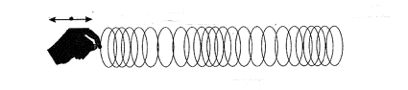
\includegraphics[width=7.691cm,height=1.693cm]{Pictures/10000001000001980000005A57BF3FA5614CAA87.png}
  Produisons
  des ondes le long d'un ressort en réalisant un mouvement vibratoire
  horizontal avec la main (l'oscillateur harmonique). Nous voyons une
  succession de compressions dilatations qui se propagent le long du
  ressort (le milieu).
\item  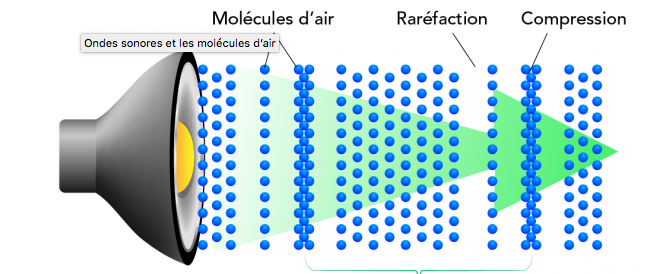
\includegraphics[width=7.103cm,height=2.916cm]{Pictures/100000010000029C00000112A3C2AC0127D5FB85.png}
Le   son est également une onde. Un haut-parleur (l'oscillateur) produit
  des ondes en \textbf{\textbf{vibrant dans l'air (le milieu)}.} Lorsque
  le haut-parleur vibre, il pousse contre l'air ambiant. Les vibrations
  entraînent une succession de compressions et de
  \textbf{\textbf{dilatations} }de l'air. Cela provoque des zones de
  haute et de basse pression à mesure que le son se propage.
\end{itemize}

\subsection{Ondes longitudinales et transversales }

\subsubsection{Vidéos à visualiser}

\begin{enumerate}
 \item \href{https://youtu.be/6eTtMmU9sqM}{Ondes mécaniques progressives}
 \item \href{https://youtu.be/X8wx9n0mgaM}{Ondes transversales et longitudinales}
 \item \href{https://youtu.be/mq9qbbSGgos}{Cours de physique TS ondes}
\item \href{https://youtu.be/cNXP3XnS60s}{45 épic battles}
\end{enumerate}

\subsection{Caractéristiques des ondes progressives}

\subsubsection{Fréquence d'une onde progressive}

Considérons une onde progressive se déplaçant au sein d'un milieu. (Par
exemple des vagues à la surface de l'eau).

Chaque point du milieu oscille avec la même fréquence que celle de
l'oscillateur harmonique responsable de la production de l'onde.

\subsubsection{Longueur d'onde d'une onde progressive }

La vitesse v d'une onde \textbf{(aussi appelée célérité} de l'onde) sera
égale au rapport de la distance parcourue par l'onde sur le temps mis
pour parcourir cette distance.

Si nous considérons un intervalle de temps égal à la période, la
distance parcourue sera alors appelée la longueur d'onde et représentée
par le lettre lambda $\lambda$.

\begin{figure}
\centering
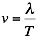
\includegraphics[width=1.011cm,height=1.011cm]{Pictures/100000010000002500000025CFFC3028DD656A44.png}
\caption{}
\end{figure}

Nous avons donc~:

\subsection{Vidéos à visualiser}

\begin{enumerate}
 \item \href{https://youtu.be/4dnzEEHRTEI}{Grandeurs et caractéristiques d'une
onde}
 \item \href{https://youtu.be/2ww9MBD9UC0}{Longueur d'onde et fréquence}
 \item  \href{https://youtu.be/C5woKhTTKCM}{Caractéristiques des ondes progressives}
\href{https://youtu.be/pkv9OIHOmSU}{Vitesse du son}
\end{enumerate}

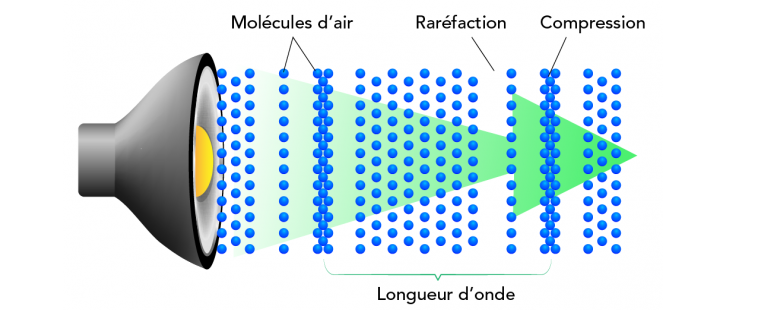
\includegraphics[width=5.913cm,height=2.417cm]{Pictures/100000010000030600000136256A22B2EA4BE45D.png}

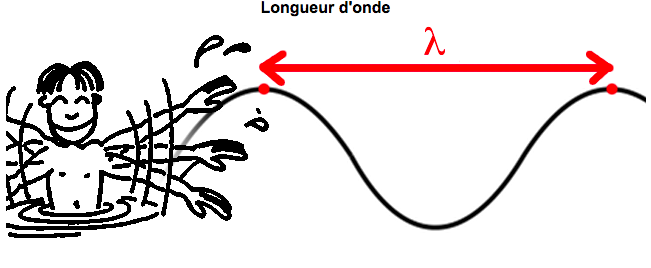
\includegraphics[width=6.668cm,height=2.748cm]{Pictures/100000010000028B0000010CEC2C8A290864C23E.png}

\subsubsection{Vitesse de propagation d'une onde }

La vitesse de propagation d'une onde ne dépend que des caractéristiques du milieu
au sein duquel l'onde se propage. 

La vitesse d'une onde au sein d'un milieu sera d'autant plus
grande que la rigidité du milieu sera importante.

Exemples~: 
\begin{enumerate}
\item  la vitesse de propagation du son dans l'air à 15°C est de 340 m/s. (à connaître par cœur)~. Nous utiliserons souvent cette valeur dans la suite du cours et
  pour les exercices.
\item  la vitesse de propagation du son dans l'air à 30°C est de 349 m/s.
\item  la vitesse de propagation du son dans l'air à 0°C est de 331 m/s.
\item  la vitesse de propagation du son dans l'eau de mer est de 1500m/s.
\end{enumerate}

Autrement dit, si vous modifiez la fréquence d'une onde sans modifier le
milieu au sein duquel elle se propage, la vitesse de l'onde reste
inchangée, c'est la longueur d'onde qui varie.

\subsection{Exercice}

\subsubsection*{Exercice 1}
  Une onde progressive transversale et entretenue est produite le long
  d'une corde. La distance entre deux crêtes est de 20 cm et la
  fréquence du vibreur étant de 50 Hz, quelle est la vitesse de
  propagation de l'onde le long de la corde. Exprime-la en km/h.
\begin{figure}
\centering
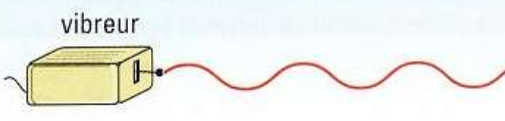
\includegraphics[width=6.468cm,height=1.552cm]{Pictures/10000001000001F900000079C23D6065BA9505A8.png}
\caption{}
\end{figure}

\begin{figure}
\centering
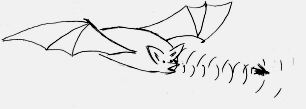
\includegraphics[width=7.103cm,height=2.54cm]{Pictures/10000001000001320000006DEEEFAD8D2B8AA8D8.png}
\caption{}
\end{figure}

\subsubsection*{Exercice 2}
  Une chauve-souris émet des ondes ultrasonores dont la plus petite
  longueur d'onde est de 3,4 mm. La durée mise par les ondes pour
  revenir à la chauve-souris permet à cette dernière, après réflexion de
  l'onde sur une proie, d'apprécier la distance la séparant de cette
  proie, un papillon par exemple. C'est le phénomène d'écholocation.

  Calcule la fréquence des ondes émises par la chauve-souris.

\subsubsection*{Exercice 3}

\begin{figure}
\centering
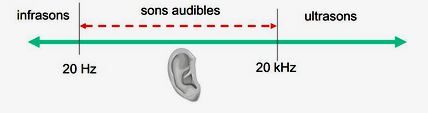
\includegraphics[width=7.996cm,height=2.281cm]{Pictures/10000001000001AC00000071A28062AB920FD735.png}
\caption{}
\end{figure}

  Sachant que la gamme d'audibilité de l'oreille humaine est comprise
  entre 20 Hz et 20 kHz, vérifie que la fréquence des ondes ultrasonores
  émises par la chauve-souris ne sont pas audibles par l'homme.

\begin{figure}
\centering
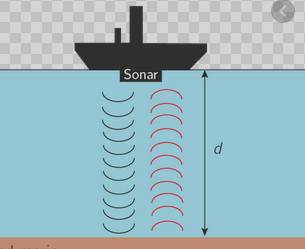
\includegraphics[width=4.186cm,height=3.41cm]{Pictures/1000000100000131000000F942C9C097631D2C4A.png}
\caption{}
\end{figure}

\subsubsection*{Exercice 4}

  Un sonar sur un bateau émet des ultrasons. L'appareil envoie un signal
  au fond de la mer. Le signal réfléchi est reçu 0,2 secondes après
  l'émission. Calculer la profondeur de l'eau.

\subsubsection*{Exercice 5}

  Une cuve à onde est un récipient rempli d'eau. Un vibreur produit des
  vagues à la surface de l'eau et à l'aide d'un miroir qui se trouve à
  l'intérieur de la cuve, nous pouvons visualiser la propagation des
  vagues sur un écran. Les cercles en traits pointillés représentent les
  creux des vagues et les cercles en traits pleins, les crêtes des
  vagues.

\subsubsection*{Exercice 6}

Un expérimentateur observe une distance entre deux crêtes de 3 cm
lorsque le vibreur oscille à une fréquence de 220 Hz.
\begin{enumerate}
\item  Quelle est la longueur d'onde de l'onde produite~?
\item   Quelle est la vitesse des ondes à la surface de l'eau (donc la vitesse
  des vagues)~?
\item  Si la fréquence du vibreur augmente, comment varie la vitesse des
  ondes~? Justifie ta réponse.
\end{enumerate}

\begin{figure}
\centering
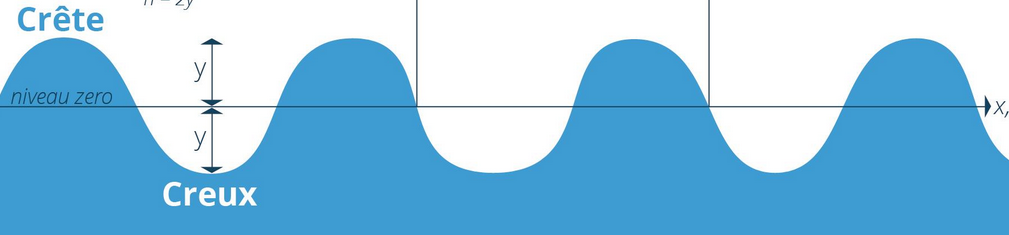
\includegraphics[width=8.255cm,height=2.046cm]{Pictures/10000001000003F1000000EBCBD13793EBF001E8.png}
\caption{}
\end{figure}

\subsubsection*{Exercice 7}

  Un bateau au mouillage, soumis à la houle des vagues, monte et descend
  de 2 mètres (en tout) toutes les 12 secondes. On mesure la distance
  entre deux crêtes qui est 8 mètres.

\begin{enumerate}
\item  Réaliser le graphique de la variation de l'élongation en fonction du
  temps.
\item  Réaliser le graphique de la variation de l'élongation en fonction de
  la distance à la source.
\item  Calculer la vitesse des vagues.
\end{enumerate}

%\hypertarget{exercice-son-8}
\subsubsection*{Exercice 8}\label{exercice-son-8}

Les affirmations suivantes sont-elles vraies ou fausses~? Indique la
réponse correcte, V ou F, et justifie chaque réponse par une petite phrase ou 
un calcul.
\begin{enumerate}
\item
  La longueur d'onde d'un son dans l'air est d'autant plus petite que la
  fréquence de l'onde est grande.
\item
  Les rides provoquées à la surface de l'eau par un excitateur sont des
  ondes longitudinales.
\item
  Un signal dont la période est de 25 ns a une fréquence de 40 GHz.
\item
  La vitesse de propagation d'une onde au sein d'un milieu dépend de la
  fréquence du signal responsable de la propagation des ondes.
\item
  Au plus une corde de guitare est tendue, au plus le son émis par cette
  corde est grave.
\item
  Le phénomène de résonance réalisé à l'aide de deux diapasons peut se
  produire dans le vide.
\item
  La longueur d'onde d'une vibration sonore dans l'air étant de 5 cm, la
  fréquence correspondante est de 6,8 kHz.
\item
  Un son d'une fréquence de 30 MHz est audible pour l'homme.
\item
  Si on entend l'écho d'un cri 3 secondes après l'avoir émis, l'obstacle
  réfléchissant se trouve donc à 510 m.
\item
  Un son aigu dans l'air a une plus grande longueur d'onde que le son
  produit par la même source mais placée dans l'eau.
\item
  Des vagues à la surface de l'eau dans une cuve à onde se déplacent
  plus rapidement si la fréquence du vibreur augmente
\end{enumerate}

%\hypertarget{exercice-9}
\subsubsection*{Exercice 9 }
\label{exercice-9-son}
Lors de la propagation d'une onde mécanique, il y a~: 
  \begin{itemize} 
       \item   Transport d'énergie
       \item   Transport de matière
       \item  Ni transport de matière et ni transport d'énergie
   \end{itemize}
Quelle(s) est (sont) la (les) affirmation(s) correcte(s)~?

\subsubsection*{Exercice 10}
  Dans une piscine, Juliette se trouve en un point M situé à 5,0
  m de la machine à vagues placée en S. Comme elle est juste assez
  grande pour sortir la tête de l'eau, elle doit sauter à chaque fois
  qu'une crête de vague l'atteint. La vitesse des vagues est de 2,0 m/s.
  Juliette doit sauter~: 
\begin{enumerate}
\item
  2,5 s après la création de la vague en S
\item
  0,40 s après la création de la vague en S
\item
  En même temps que se crée la vague en S
\end{enumerate}

\subsubsection*{Exercice 11}
Les ondes progressives périodiques présentent~: 
\begin{enumerate}
\item  Une périodicité temporelle
\item  Une périodicité spatiale
\end{enumerate}
La fréquence d'un phénomène périodique~: 
\begin{enumerate}
\item est l'inverse de la période
\item est le nombre de fois que se répète le phénomène par seconde
\item représente la durée du phénomène
\end{enumerate}


\subsubsection*{Exercice 12}

Une onde de période T = 10 ms se propage à la vitesse v = 250 \si{ m/s}. Sa longueur d'onde $\lambda$ vaut~: 
\begin{enumerate}
\item  2,5 \si{m}
\item
  2,5 km
\item
  25 km
\end{enumerate}

\subsubsection*{Exercice 13}

Voici quatre propositions concernant la propagation du son
  dans l'air, laquelle (lesquelles) est (sont) correcte(s)~?

\begin{enumerate}
\item  Il s'agit de la transmission de proche en proche de la vibration des
  molécules constituant l'air.
\item  Cette vibration s'effectue perpendiculairement à la direction de
  propagation.
\item  La longueur d'onde d'un son périodique est indépendante de sa
  fréquence.
\item  Dans le même milieu, un observateur entend les sons aigus plus
  rapidement que les sons graves issus simultanément de la même source.
\end{enumerate}

\subsubsection*{Exercice 14}

On utilise des ultrasons émis à la fréquence de 40 \si{kHz}, dans
  l'air. Parmi les affirmations suivantes, laquelle (lesquelles) est
  (sont) correcte(s)~?
\begin{enumerate}
\item  La longueur d'onde des ultrasons est 8,5 \si{mm}.
\item
  La distance parcourue pendant une période est 8,5 \si{mm}.
\item  La fréquence est modifiée si l'on change la nature du gaz dans lequel
  ils se propagent.
\item  Si la fréquence des ultrasons est divisée par deux, alors leur vitesse
  de propagation dans un milieu donné est également divisée par 2.
\end{enumerate}


\section{Étude mathématique de l'onde progressive}

\subsection{Vidéos à visualiser}
\begin{enumerate}
 \item \href{https://youtu.be/9Hs9jeuDzwg}{Onde mécanique sinusoïdale dans une corde }
 \item \href{https://youtu.be/N654RoNHalc}{Onde sur une corde.}
\end{enumerate}

\subsection{Mise en situation~: }

Soit une onde transversale progressive et périodique produite le long
d'une corde.
\begin{figure}
\centering
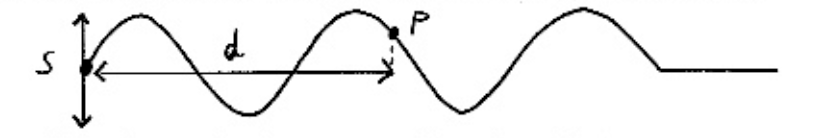
\includegraphics[width=13.645cm,height=2.305cm]{Pictures/10000001000003340000008AA6B62AF7250A4682.png}
\caption{}
\end{figure}

\begin{itemize}
\item
  S étant la source (le vibreur est un oscillateur harmonique).
\item
  P est un point de la corde situé à une distance d de la source.
\item
  Vous savez que la variation de l'élongation de la source S en fonction
  du temps peut s'écrire~:
\end{itemize}

y\textsubscript{s}(t) = A sin (t ) si nous considérons la constante de
phase nulle.

Comment pourrions-nous écrire la variation de l'élongation d'un point
  P de la corde en fonction du temps, sachant que le point P est distant
  d'une distance d de la source~? Notons la $y_P(t)$.

Un point P quelconque de la corde oscille à la même fréquence que la
source S mais à un instant donné, leurs élongations ne sont pas les
mêmes. Le point P oscille comme la source mais avec un certain déphasage
dû au temps que met l'onde pour atteindre le point P. Le point P oscille
donc avec un certain retard par rapport à la source S.

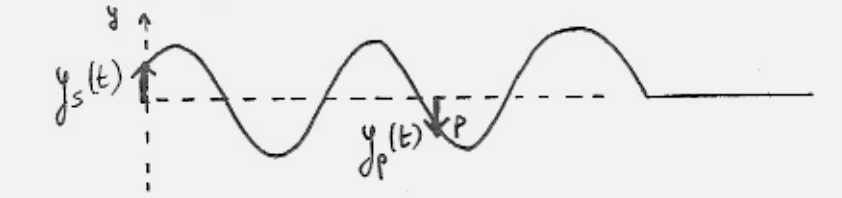
\includegraphics[width=12.696cm,height=2.99cm]{Pictures/100000010000034A000000C6944A1FC3E4803CD5.png}
FIXME à faire au net

Le point P reproduit l'oscillation de la source avec un certain retard
t' qui est le temps mis par l'onde pour atteindre le point P.

Or nous savons que le temps est le rapport d'une distance sur une
vitesse.

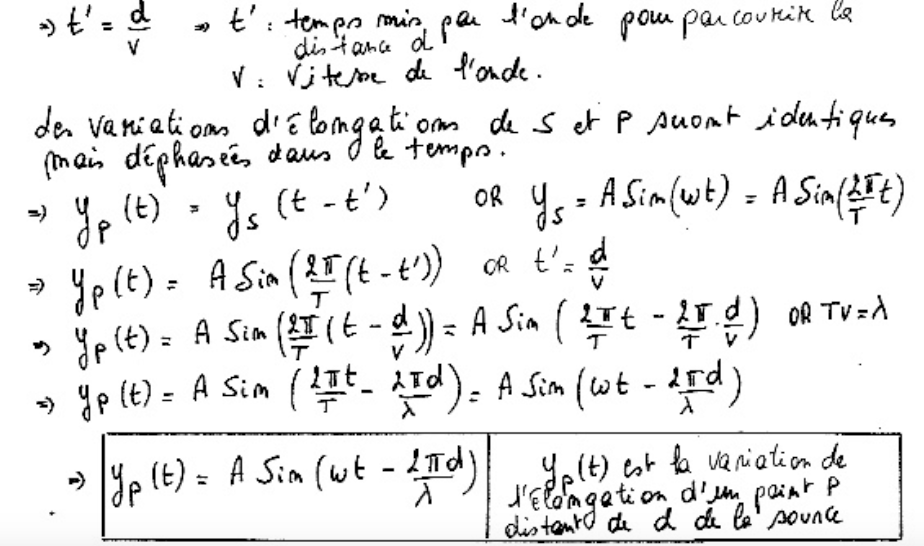
\includegraphics[width=14.152cm,height=7.717cm]{Pictures/100000010000039C0000022244D6A7EE40B9357C.png}

\subsection{Exemple}

Un vibreur provoque des ondes sinusoïdales de période T = 2s à
l'extrémité d'une corde. A l'instant initial, l'élongation est nulle.
L'amplitude des ondes est de 1 mètre. La vitesse de l'onde le long de la
corde est de 4 m/s.

\begin{enumerate}
\item  Déterminez la longueur d'onde le long de cette corde.
\item  Quelle est l'élongation du vibreur à t = 10 s~?
\item  Quelle sera la distance parcourue par l'onde à t = 10s~?
\item  Représenter la corde à t = 10 s.
\item  Quelle sera l'élongation d'un point P de la corde, situé à une
  distance d = 3m du vibreur à t = 10 s.
Vérifier l'exactitude de la réponse sur le graphique du point précédent.
\item  Quelle sera l'élongation d'un point P de la corde, situé à une
  distance d = 5m du vibreur à t = 10 s.
Vérifier l'exactitude de la réponse sur le graphique du point 4).
\end{enumerate}

\end{multicols}
